\documentclass{article}

\usepackage{amsmath}
\usepackage{amsfonts} % For math fonts.
\usepackage{amssymb} % For other math symbols not covered by amsmath.
\usepackage[pdftex]{graphicx} % For pictures, use \includegraphics[scale=decimal]{pic.png}; must be a .png file type.
\usepackage{multicol}
\usepackage{textcomp}
\usepackage[colorlinks = true, urlcolor = blue]{hyperref}
\usepackage{enumitem}
\usepackage{graphbox} 
\usepackage{subfig}
\usepackage{multicol}
\usepackage{nopageno}
\usepackage{bm}


\usepackage{tikz}
\usetikzlibrary{positioning, calc}
\usetikzlibrary{shapes.geometric,angles,quotes}
\usepackage{tikz-3dplot}


%page formatting
\usepackage{fullpage}
\setlength{\parindent}{0pt}


\newcommand{\tab}{\hspace*{0.25in}}
\newcommand{\csq}[1]{\reflectbox{''}#1''}  %This produces CS style quotes.
\newcommand{\csqt}[1]{\text{\reflectbox{''}#1''}}  %This produces CS style quotes as text.


\usepackage{listings}
\lstset
{ %Formatting for code in appendix
    language=Python,
    basicstyle=\footnotesize,
    numbers=left,
    stepnumber=1,
    showstringspaces=false,
    tabsize=2,
    breaklines=true,
    breakatwhitespace=false,
}


\begin{document}



%split_point

%\end{document}
Lone Star \hfill Basic IO quiz\\
section 4\\
\begin{enumerate}
\item (1.1) Write a program that asks the user for \\
		\begin{minipage}{0.5\textwidth}	
		\vspace*{-0.5em}
			\begin{enumerate}  \setlength\itemsep{-0.3em}
				\item the year,
				\item the month, and
				\item the day	
			\end{enumerate} \vspace*{-1ex}
		and then outputs the date.
		\end{minipage}
		%\
		\begin{minipage}{0.5\textwidth}
			\centering
			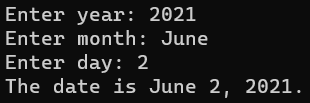
\includegraphics[scale=0.75]{./imgs/dateOutput.png}\\
			Your output should be similar to this.
		\end{minipage}

	

\item (1.2) 
		Write a program that asks the user for \\
		\begin{minipage}{0.5\textwidth}
		\vspace*{-0.5em}
			\begin{enumerate}  \setlength\itemsep{-0.3em}
				\item their first name and
				\item their last name.  
			\end{enumerate} \vspace*{-1ex}
		and then outputs a greeting.
		\end{minipage}
		%\
		\begin{minipage}{0.5\textwidth}
			\centering
			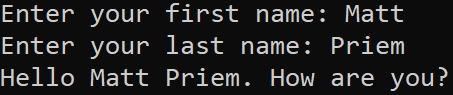
\includegraphics[scale=0.9]{./imgs/outputGreeting.png}\\
			Your output should be similar to this.
		\end{minipage}

%end_of_questions

\item (1.3) 
		Write code to swap the values of $x$ and $y$ using a temporary variable and without using
		the built-in function swap().\\		
		\begin{tabular}{|ll}
			\\			
			x = 3\\
			y = 7\\[5pt]
			\#Your code here. \\[5pt]
			& \\ & \\ & \\ & \\ & \\ & \\ & \\ & \\ & \\ & \\ 
		\end{tabular}


%end_of_questions

\end{enumerate}
\pagebreak
Dot Matrix \hfill Basic IO quiz\\
section 5\\
\begin{enumerate}
\item (1.1) Write a program that asks the user for \\
		\begin{minipage}{0.5\textwidth}	
		\vspace*{-0.5em}
			\begin{enumerate}  \setlength\itemsep{-0.3em}
				\item the year,
				\item the month, and
				\item the day	
			\end{enumerate} \vspace*{-1ex}
		and then outputs the date.
		\end{minipage}
		%\
		\begin{minipage}{0.5\textwidth}
			\centering
			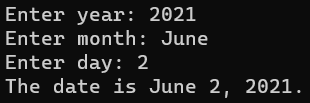
\includegraphics[scale=0.75]{./imgs/dateOutput.png}\\
			Your output should be similar to this.
		\end{minipage}

	

\item (1.2) 
		Write a program that asks the user for \\
		\begin{minipage}{0.5\textwidth}
		\vspace*{-0.5em}
			\begin{enumerate}  \setlength\itemsep{-0.3em}
				\item their first name and
				\item their last name.  
			\end{enumerate} \vspace*{-1ex}
		and then outputs a greeting.
		\end{minipage}
		%\
		\begin{minipage}{0.5\textwidth}
			\centering
			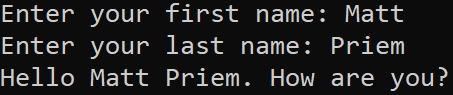
\includegraphics[scale=0.9]{./imgs/outputGreeting.png}\\
			Your output should be similar to this.
		\end{minipage}

%end_of_questions

\item (1.3) 
		Write code to swap the values of $x$ and $y$ using a temporary variable and without using
		the built-in function swap().\\		
		\begin{tabular}{|ll}
			\\			
			x = 3\\
			y = 7\\[5pt]
			\#Your code here. \\[5pt]
			& \\ & \\ & \\ & \\ & \\ & \\ & \\ & \\ & \\ & \\ 
		\end{tabular}


%end_of_questions

\end{enumerate}
\pagebreak
Dark Helmet \hfill Basic IO quiz\\
section 4\\
\begin{enumerate}
\item (1.1) Write a program that asks the user for \\
		\begin{minipage}{0.5\textwidth}	
		\vspace*{-0.5em}
			\begin{enumerate}  \setlength\itemsep{-0.3em}
				\item the year,
				\item the month, and
				\item the day	
			\end{enumerate} \vspace*{-1ex}
		and then outputs the date.
		\end{minipage}
		%\
		\begin{minipage}{0.5\textwidth}
			\centering
			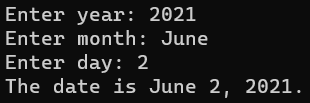
\includegraphics[scale=0.75]{./imgs/dateOutput.png}\\
			Your output should be similar to this.
		\end{minipage}

	

\item (1.2) Write a program that asks the user for \\
		\begin{minipage}{0.5\textwidth}
		\vspace*{-0.5em}
			\begin{enumerate}  \setlength\itemsep{-0.3em}
				\item their first name and
				\item their age.  
			\end{enumerate} \vspace*{-1ex}
		and then outputs a greeting.
		\end{minipage}
		%\
		\begin{minipage}{0.5\textwidth}
			\centering
			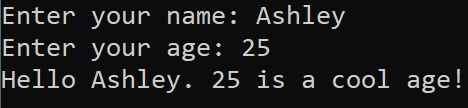
\includegraphics[scale=0.95]{./imgs/outputGreetingWithAge.png}\\
			Your output should be similar to this.
		\end{minipage}




\item (1.3) 
		Write code to swap the values of $x$ and $y$ using a temporary variable and without using
		the built-in function swap().\\		
		\begin{tabular}{|ll}
			\\			
			x = 3\\
			y = 7\\[5pt]
			\#Your code here. \\[5pt]
			& \\ & \\ & \\ & \\ & \\ & \\ & \\ & \\ & \\ & \\ 
		\end{tabular}


%end_of_questions

\end{enumerate}
\pagebreak
President Skroob \hfill Basic IO quiz\\
section 1\\
\begin{enumerate}
\item (1.1) Write a program that asks the user for \\
		\begin{minipage}{0.5\textwidth}	
		\vspace*{-0.5em}
			\begin{enumerate}  \setlength\itemsep{-0.3em}
				\item the year,
				\item the month, and
				\item the day	
			\end{enumerate} \vspace*{-1ex}
		and then outputs the date.
		\end{minipage}
		%\
		\begin{minipage}{0.5\textwidth}
			\centering
			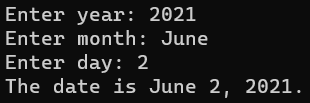
\includegraphics[scale=0.75]{./imgs/dateOutput.png}\\
			Your output should be similar to this.
		\end{minipage}

	

\item (1.2) Write a program that asks the user for \\
		\begin{minipage}{0.5\textwidth}
		\vspace*{-0.5em}
			\begin{enumerate}  \setlength\itemsep{-0.3em}
				\item their first name and
				\item their age.  
			\end{enumerate} \vspace*{-1ex}
		and then outputs a greeting.
		\end{minipage}
		%\
		\begin{minipage}{0.5\textwidth}
			\centering
			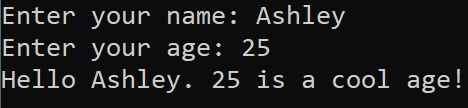
\includegraphics[scale=0.95]{./imgs/outputGreetingWithAge.png}\\
			Your output should be similar to this.
		\end{minipage}




\item (1.3) 
		Write code to swap the values of $x$ and $y$ using a temporary variable and without using
		the built-in function swap().\\		
		\begin{tabular}{|ll}
			\\			
			x = 3\\
			y = 7\\[5pt]
			\#Your code here. \\[5pt]
			& \\ & \\ & \\ & \\ & \\ & \\ & \\ & \\ & \\ & \\ 
		\end{tabular}


%end_of_questions

\end{enumerate}
\pagebreak
\end{document}